\documentclass[]{antpostershort}
\usepackage{graphicx}                                                      % control over the import of graphics
\usepackage[table,dvipsnames]{xcolor}                                      % Define tables (with colour control)
\usepackage{float}                                                         % Control over graphics + tables float
\usepackage[justify]{ragged2e}                                             % control over text alignment
\usepackage{booktabs}                                                      % caption graphics + tables (with name in bold)
\usepackage[labelfont=bf]{caption} 
\usepackage{subcaption}
\usepackage{tikz}
\usetikzlibrary{shapes,decorations,decorations.pathreplacing,arrows,calc,arrows.meta,fit,positioning}
\tikzset{
    auto,node distance =1 cm and 1 cm,semithick,
    state/.style ={ellipse, draw, minimum width = 0.7 cm},
    point/.style = {circle, draw, inner sep=0.04cm,fill,node contents={}},
    bidirected/.style={Latex-Latex,dashed},
    el/.style = {inner sep=2pt, align=left, sloped}
}
\usepackage{mathtools}                                                     % Various maths functions
\usepackage{amssymb}                                                       % Various maths functions
\usepackage{amsmath}                                                       % Various maths functions
\usepackage{dsfont}                                                        % Various maths functions
\usepackage{centernot}                                                     % center \not usage
\usepackage{siunitx} \sisetup{round-mode=places, round-precision=3}        % Formalise use of units and numbers among text
\usepackage{amsthm}                                                        % NEvrionemtn for theorems.
\DeclareMathOperator{\eps}{\varepsilon}                                    % epsilon short hand shortcut
\renewcommand{\vec}[1]{\boldsymbol{\mathit{#1}}}                           % vector notation shortcut
\newcommand{\mat}[1]{\boldsymbol{\mathit{#1}}}                             % matrix notation shortcut
\newcommand{\Prob}[1]{\Pr\left( #1 \right)}                         % SHortcut for probability notation
\newcommand{\Probgiven}[2]{\Pr\left( #1 \, \middle\vert \, #2 \right)} % SHortcut for probability notation, given
\newcommand{\E}[2][]{\mathbb{E}_{#1} \left[ #2 \right]}                    % Expectation (with optional subscript) shortcut
\newcommand{\Egiven}[3][]{\mathbb{E}_{#1} \left[ #2 \, \middle\vert \, #3 \right]} % Expectation given (with optional subscript) shortcut
\newcommand{\Var}[2][]{\text{Var}_{#1} \left( #2 \right)}                  % Variation (with optional subscript) shortcut
\newcommand{\Cov}[1]{\text{Cov} \left( #1 \right)}                         % Covariance (with optional subscript) shortcut
\newcommand{\indicator}[1]{\mathds{1}\left\{ #1 \right\}}                  % SHortcut for indicator function
\renewcommand{\hat}[1]{\widehat{#1}}                                       % Default estimator notation is widehat
\renewcommand{\bar}[1]{\overline{#1}}                                      % Make over bar look nicer
\renewcommand{\tilde}[1]{\widetilde{#1}}                                   % Make over tilde look better
\newcommand{\indep}{\, \raisebox{0.05em}{\rotatebox[origin=c]{90}{$\models$}} \,}% Statistical independence symbol.

% Poster metadata
\title{Causal Mediation in Natural Experiments}
\author{Senan Hogan-Hennessy}
\logo{../presentation-files/cornell-reduced/cu-seal-large.png}
% Multiple lines must be separated by '\?'.
\qrdata{https://raw.githubusercontent.com/shoganhennessy/mediation-natural-experiment/main/mediation-natural-experiment-2025.pdf}
\abstract{
    Conventional CM assumes away choice.\\
    My \textbf{MTE approach} puts \textbf{choice back} into the equation.
}

\begin{document}
\maketitle

\vskip-0.5cm
%\section{Abstract}
%
%Natural experiments provide settings for estimating causal effects, but give little indication of the mechanisms involved.
%My paper develops a Causal Mediation (CM) method that accounts for individuals' choices of a mediator mechanism --- such as whether to use healthcare or attend college --- using instrumental variation in mediator costs.
%Applying it to the Oregon Health Insurance Experiment (OHIE) shows that the effect of access to socialised healtcare effect on well-being operates through increased healthcare use, with notable direct effects.

\section{Research Question}

\begin{enumerate}
    \item How can we identify mechanisms in natural experiments --- when individuals freely choose a mediating mechanism? \\
    \textit{Conventional CM breaks down when mediator choice is unconstrained, giving biased inference.}

    \item Can we model the system to deliver unbiased CM estimates? \\
    \textit{I develop a Marginal Treatment Effect (MTE) approach, treating a mediator as a choice shaped by incentives, not assuming it is random.}

    \item What mechanisms explain the effects of access to socialised healthcare in the Oregon Health Insurance Experiment? \\
    \textit{I compare conventional CM to my MTE approach estimating the role of increased healthcare take-up in the effect of new access to socialised health insurance.}
\end{enumerate}

%\section{Contribution \& Literature}
%
%I show that conventional CM methods, break down in economic settings where mediators are chosen rather than randomly assigned.
%I formalise the resulting selection biases on the average direct and indirect effects, then develop a CM framework consistent with economic models of selection --- linking CM to the MTE literature.
%This bridges the practice of suggestive evidence for mechanisms to a rigorous identification strategy for mechanism effects under endogenous mediator choice.

\section{Oregon Health Insurance Experiment (OHIE)}

\begin{figure}[H]
    \begin{subfigure}[t]{0.475\textwidth}
        \centering
        \caption{Causal Model: Suggestive Evidence.}
        %\vskip0.2cm
        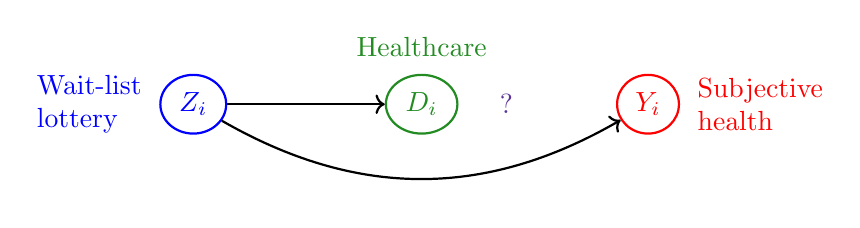
\begin{tikzpicture}
            \node[state,thick,ForestGreen] (mediator) at (0,0) {$D_i$};
            \node[state,thick,blue] (treatment) [left=2cm of mediator] {$Z_i$};
            \node[state,thick,red] (outcome)   [right=2cm of mediator] {$Y_i$};
            % Label Z_i, D, Y_i
            \node[color=ForestGreen] [above=0.1cm of mediator] {Healthcare};
            \node[color=blue,align=left] [left=0.1cm of treatment] {Wait-list \\ lottery};
            \node[color=red,align=left] [right=0.1cm of outcome] {Subjective \\ health};
            % Draw the causal arrows
            \path[->, thick] (treatment) edge (mediator);
            %\path[->, dashed,color=gray] (mediator) edge (outcome);
            \path[->, thick] (treatment) edge[bend right=30] (outcome);
            % Label the problem.
            \node[color=RoyalPurple] [right=0.4cm of mediator] {?};
        \end{tikzpicture}
        \justify
        Suggestive evidence for mechanisms $\implies$ necessary (not sufficient) evidence on healthcare as mediating mechanism.
    \end{subfigure}
    \begin{subfigure}[t]{0.475\textwidth}
        \centering
        \caption{Causal Model: MTE Approach.}
        %\vskip0.2cm
        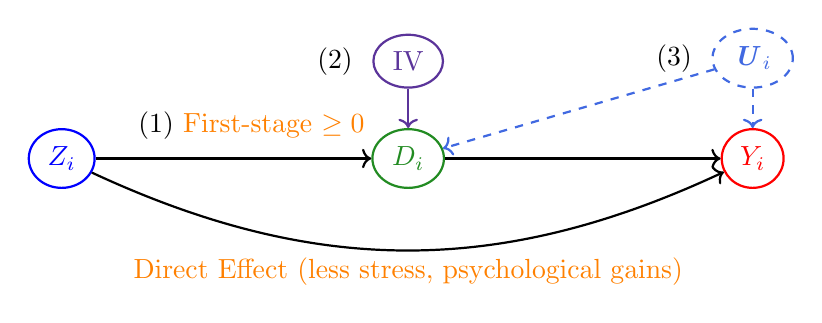
\begin{tikzpicture}
            \node[state,thick,ForestGreen] (mediator) at (0,0) {$D_i$};
            \node[state,thick,blue] (treatment) [left=3.5cm of mediator] {$Z_i$};
            \node[state,thick,red] (outcome)   [right=3.5cm of mediator] {$Y_i$};
            % Label Z_i, D, Y_i
            % Draw the causal arrows
            \path[->, thick] (treatment) edge (mediator);
            \path[->, thick] (mediator) edge (outcome);
            \path[->, thick] (treatment) edge[bend right=25] (outcome);
            \node[state, thick,dashed,thick,RoyalBlue] (confounderU) [
                above=0.5cm of outcome] {$\vec U_i$};
            % Label direct and indirect effects
            %\node[color=orange] [above right=-0.3cm and 0.75cm of mediator] {Indirect};
            \node[color=orange] [below=0.75cm of mediator] {Direct Effect (less stress, psychological gains)};
            \node[align=left] [above left=-0.15cm and 0.1cm of mediator] {
                (1) \textcolor{orange}{First-stage $\geq 0$}};
            \node[left=0.125cm of confounderU] {(3)};
            \path[->,thick,dashed,color=RoyalBlue] (confounderU) edge (mediator);
            \path[->,thick,dashed,color=RoyalBlue] (confounderU) edge (outcome);
            \node[state,thick,RoyalPurple] (instrument) [above=0.5cm of mediator] {IV};
            \path[->,thick,color=RoyalPurple] (instrument) edge (mediator);
            \node [left=0.125cm of instrument] {(2)};
        \end{tikzpicture}
        \justify
        MTE model with assumptions (1) mediator monotonicity, (2) cost-shift IV, (3) relevant selection $\implies$ sufficient evidence.
    \end{subfigure}
\end{figure}
\vskip-0.5cm
\par\noindent\rule{\textwidth}{0.4pt}
\vskip-0.25cm
\begin{figure}[H]
    \begin{subfigure}[t]{0.475\textwidth}
        \centering
        \caption{Total Effects of the OHIE.}
        %\vskip0.2cm
        \includegraphics[width=\textwidth]{
            ../presentation-files/figures/insurance-effects.png}
        \begin{itemize}
            \item Suggestive evidence $\to$ healthcare mediates OHIE gains
            \item Unknown percentage, and evidence is not sufficient.
        \end{itemize}
    \end{subfigure}
    \hfill
    \begin{subfigure}[t]{0.475\textwidth}
        \centering
        \caption{CM Analyses of Healthcare Take-up in the OHIE.}
        %\vskip0.2cm
        \includegraphics[width=\textwidth]{
            ../../text/sections/figures/mediation-health.png}
        \begin{itemize}
            \item Conventional CM $\to$ healthcare mediates $\approxeq$ 0\%
            \item MTE-based CM $\to$ healthcare mediates $\approxeq$ 20--80\%.
        \end{itemize}
    \end{subfigure}
\end{figure}

%The OHIE offered access to socialised health insurance by a wait-list lottery, leading to increased healthcare take-up and benefits in subjective health.
%Standard practice interprets this as evidence that healthcare use mediates benefits from socialised health insurance effects --- but this inference is so far only suggestive, and omits direct benefits such as psychological gains from no longer being uninsured.
%My method estimates these CM effects, showing that increased healthcare use explains much of the well-being gain, while direct effects remain substantial.
%This illustrates how accounting for endogenous mediator choice changes conclusions in a natural experiment setting.
\end{document}
